\documentclass[11pt,a4paper,oneside]{report}

% Informe técnico del diseño, fabricación y montaje del nodo embarcado.
% El documento es autónomo: puede compilarse desde docs/ o desde la raíz del
% repositorio porque se incluyen las dos rutas posibles para las fotografías.
\usepackage[utf8]{inputenc}
\usepackage[T1]{fontenc}
\usepackage[spanish,es-nodecimaldot]{babel}
\usepackage{lmodern}
\usepackage{microtype}
\usepackage[a4paper,margin=2.55cm,headheight=15pt]{geometry}
\usepackage{graphicx}
\graphicspath{{assets/informe_pcb_caja/}{docs/assets/informe_pcb_caja/}}
\usepackage{booktabs}
\usepackage{tabularx}
\usepackage{array}
\usepackage{float}
\usepackage{caption}
\usepackage{xcolor}
\usepackage{enumitem}
\usepackage{fancyhdr}
\usepackage{lastpage}
\usepackage{titlesec}
\usepackage{listings}
\usepackage[most]{tcolorbox}
\usepackage[hidelinks]{hyperref}

\definecolor{azulproyecto}{HTML}{123B5D}
\definecolor{turquesa}{HTML}{0B7A75}
\definecolor{azulclaro}{HTML}{EAF4F4}
\definecolor{gristexto}{HTML}{38434D}
\definecolor{grisfila}{HTML}{F4F7F9}
\definecolor{verde}{HTML}{1B8F5A}
\definecolor{ambar}{HTML}{B86B00}
\definecolor{rojo}{HTML}{B33A45}

\hypersetup{
  colorlinks=true,
  linkcolor=azulproyecto,
  urlcolor=turquesa,
  citecolor=azulproyecto,
  pdftitle={Diseño, fabricación y montaje de la PCB y la caja del nodo embarcado},
  pdfauthor={Proyecto de monitoreo vehicular}
}

\setlength{\parindent}{0pt}
\setlength{\parskip}{0.55em}
\setlength{\emergencystretch}{3em}
\setlist[itemize]{leftmargin=1.45em,itemsep=0.22em,topsep=0.28em}
\setlist[enumerate]{leftmargin=1.7em,itemsep=0.28em,topsep=0.28em}
\renewcommand{\arraystretch}{1.18}

\titleformat{\chapter}[display]
  {\normalfont\bfseries\color{azulproyecto}}
  {\filleft\Large\chaptername\ \thechapter}
  {0.5ex}{\titlerule[1.2pt]\vspace{1ex}\Huge}
\titleformat{\section}{\Large\bfseries\color{azulproyecto}}{\thesection}{0.72em}{}
\titleformat{\subsection}{\large\bfseries\color{turquesa}}{\thesubsection}{0.72em}{}

\captionsetup{font=small,labelfont=bf,justification=centering}

\pagestyle{fancy}
\fancyhf{}
\fancyhead[L]{\small\color{gristexto}Proyecto de monitoreo vehicular}
\fancyhead[R]{\small\color{gristexto}PCB, caja y montaje}
\fancyfoot[C]{\small\thepage\ de \pageref{LastPage}}
\renewcommand{\headrulewidth}{0.35pt}
\renewcommand{\footrulewidth}{0pt}

\lstdefinestyle{codigo}{
  basicstyle=\ttfamily\small,
  backgroundcolor=\color{grisfila},
  frame=single,
  rulecolor=\color{azulclaro},
  breaklines=true,
  columns=fullflexible,
  keepspaces=true,
  showstringspaces=false,
  keywordstyle=\color{azulproyecto}\bfseries,
  commentstyle=\color{gristexto}\itshape
}
\lstset{style=codigo}

\newcommand{\codigo}[1]{\texttt{\small #1}}
\newcommand{\implementado}{\textcolor{verde}{\textbf{Implementado}}}
\newcommand{\visual}{\textcolor{verde}{\textbf{Validado visualmente}}}
\newcommand{\automatico}{\textcolor{azulproyecto}{\textbf{Validado automáticamente}}}
\newcommand{\pendiente}{\textcolor{ambar}{\textbf{Pendiente}}}

\newtcolorbox{evidenciabox}[1][]{
  enhanced,breakable,colback=azulclaro,colframe=turquesa,
  boxrule=0.7pt,arc=1.5mm,left=3mm,right=3mm,top=2mm,bottom=2mm,#1
}
\newtcolorbox{alertabox}[1][]{
  enhanced,breakable,colback=red!3,colframe=rojo,
  boxrule=0.7pt,arc=1.5mm,left=3mm,right=3mm,top=2mm,bottom=2mm,#1
}

\begin{document}

\pagenumbering{roman}

\chapter*{Resumen}
\addcontentsline{toc}{chapter}{Resumen}

Este informe documenta la conversión del diseño electrónico del nodo embarcado en
un conjunto físico compuesto por una PCB portadora, los módulos de adquisición y
comunicación, y una caja fabricada mediante impresión 3D en PETG. Se describe la
secuencia completa: definición de interfaces a partir del firmware, captura del
esquemático en KiCad, distribución de la tarjeta, orden de fabricación, inspección,
soldadura, diseño mecánico, impresión, fijación y montaje final.

La tarjeta se planteó como una portadora modular. El ESP32 se mantiene desmontable
mediante zócalos y los sensores se conectan por cabeceras identificadas. Esta
decisión reduce el riesgo de dañar el microcontrolador durante las pruebas y permite
reemplazar un módulo sin rehacer la placa. La caja protege la electrónica, deja
accesibles la alimentación y el USB, y añade ventilación y puntos de fijación para
que el conjunto pueda trasladarse como una sola unidad.

Las once figuras de este informe provienen del documento de imágenes entregado para
este informe. Se utilizan como evidencia visual del flujo de diseño, fabricación y
ensamblaje. Las cotas numéricas de la caja no se reproducen aquí: la geometría se
ajustó sobre la revisión mecánica realmente impresa y cualquier medida heredada de
una versión anterior queda expresamente fuera de este documento.

\begin{evidenciabox}
\textbf{Resultado del trabajo.} Existe una revisión física fotografiada de la PCB
con sus headers, alimentación y capacitor de reserva, una caja PETG impresa y un
montaje final en el que se comprueba el encaje de la placa, el acceso frontal y la
separación de los módulos. La evidencia funcional de cada sensor debe leerse junto
con la secuencia de bring-up y los límites indicados en el capítulo~\ref{chap:validacion}.
\end{evidenciabox}

\tableofcontents
\clearpage
\pagenumbering{arabic}

% -----------------------------------------------------------------------------
\chapter{Propósito, alcance y método}
% -----------------------------------------------------------------------------

\section{Propósito}

Los informes anteriores cubren la investigación, las pruebas de software y la
plataforma de comunicación. Este documento se concentra en la capa física que
permite llevar esas funciones al vehículo: la PCB que organiza el cableado y la
envolvente que sostiene, protege y hace accesible el conjunto.

El objetivo fue pasar de conexiones sobre protoboard a un ensamblaje repetible,
con referencias de conexión visibles, menor cantidad de cables sueltos y una
interfaz mecánica coherente. La PCB no reemplaza a los módulos del proyecto; los
interconecta y distribuye su alimentación respetando los límites definidos por el
firmware.

\section{Alcance}

El informe incluye:

\begin{itemize}
  \item definición eléctrica y captura del esquemático en KiCad;
  \item selección de conectores, zonas de placement y criterios de routing;
  \item fabricación de la tarjeta y revisión visual del lote fotografiado;
  \item soldadura de headers, bornera y elementos de filtrado;
  \item modelado, impresión 3D y acabado de la caja en PETG;
  \item fijación de la PCB, organización de módulos, cableado y acceso de servicio;
  \item plan de bring-up y criterios de aceptación para la integración.
\end{itemize}

No se incluyen en este informe el despliegue cloud, la precisión metrológica de los
sensores ni una certificación para uso automotriz. Tampoco se fijan dimensiones de
la caja: se evita así contaminar la revisión vigente con cotas antiguas.

\section{Fuentes de verdad y criterio de evidencia}

La asignación de pines se comprobó contra \codigo{include/pins.h}, los intervalos y
direcciones contra \codigo{include/config.h}, y la secuencia de pruebas contra
\codigo{docs/tests.md}, \codigo{docs/wiring.md} y
\codigo{docs/especificacion\_pcb.md}.
El código ejecutable tiene prioridad sobre cualquier dibujo o descripción anterior.

Para no confundir una fotografía con una prueba eléctrica, se usan cuatro niveles:

\begin{description}
  \item[\implementado.] La decisión existe en el esquema, el firmware o la
        configuración del proyecto.
  \item[\automatico.] Una compilación, prueba unitaria o revisión estática cubre
        el comportamiento sin depender de un sensor conectado.
  \item[\visual.] La fotografía proporcionada permite comprobar una pieza física,
        su orientación o su encaje. Esto no demuestra precisión ni funcionamiento
        prolongado.
\end{description}

\section{Decisión sobre las cotas de la caja}

La caja fue rediseñada y ajustada con la PCB y los módulos disponibles al momento
de imprimir. Por solicitud del proyecto, este informe no transcribe valores
numéricos de largo, ancho, alturas, taladros, holguras ni posiciones: las cotas de
versiones antiguas del repositorio no representan necesariamente la pieza actual.
La verificación que sí se conserva es funcional: los separadores coinciden con los
agujeros de la placa, los módulos entran sin forzar, los cables no quedan prensados
y los accesos de servicio permanecen disponibles.

% -----------------------------------------------------------------------------
\chapter{Requisitos e interfaz eléctrica}
% -----------------------------------------------------------------------------

\section{Requisitos de diseño}

El conjunto debía cumplir simultáneamente los siguientes requisitos:

\begin{enumerate}
  \item concentrar en una tarjeta las conexiones de sensores, memoria y
        comunicaciones;
  \item conservar el ESP32 como módulo reemplazable y mantener su USB accesible;
  \item trabajar con señales de 3,3 V y una referencia de tierra común;
  \item separar la alimentación del SIM800L de la rama de sensores;
  \item dejar espacio para antenas, micrófono y sensor de luz sin obstrucciones;
  \item permitir inspección, mantenimiento y sustitución de módulos;
  \item proteger el montaje con una caja ventilada y desmontable.
\end{enumerate}

La selección de conectores se hizo pensando en el módulo físico y no solo en el
nombre comercial. En particular, un ``ESP32 DevKit V1'' puede cambiar de contorno
entre fabricantes; por ello se utilizó la placa disponible para comprobar la
orientación y el paso de los zócalos antes del montaje.

\section{Mapa de interfaces}

La tabla~\ref{tab:pines} resume las interfaces que deben aparecer en la PCB. Los
números son GPIO reales del ESP32, no etiquetas serigrafiadas de clones.

\begin{table}[H]
\centering
\small
\caption{Interfaz de la PCB con el firmware vigente.}
\label{tab:pines}
\begin{tabularx}{\textwidth}{>{\bfseries}p{3.0cm} p{2.0cm} p{3.1cm} X}
\toprule
Módulo & Referencia & GPIO / bus & Función y criterio de conexión \\
\midrule
DHT11 & J-DHT & GPIO27 & Datos digitales; pull-up a 3,3 V si el breakout no lo incluye. \\
GPS NEO-6M & J-GPS & GPIO32/33, UART2 & TX del GPS hacia RX del ESP32; 9600 baudios. \\
GY-801 & J-GY801 & GPIO21/22, I2C & Acelerómetro, giroscopio, magnetómetro y barómetro. \\
BH1750 & J-BH1750 & GPIO21/22, I2C & Iluminancia; dirección fijada en el módulo. \\
microSD & J-SD & GPIO18/19/23/5, SPI & SCK, MISO, MOSI y CS; CS con pull-up durante el arranque. \\
SIM800L & J-SIM & GPIO16/17, UART1 & Ruta celular experimental; fuente y retorno independientes. \\
INMP441 & J-MIC & GPIO26/25/34, I2S & BCLK, WS y datos; GPIO34 se usa únicamente como entrada. \\
Alimentación & J-PWR & 5 V regulados y GND & Entrada de la portadora; no conectar directamente a batería del vehículo. \\
\bottomrule
\end{tabularx}
\end{table}

En el esquemático del lote aparecen también referencias J4 y J5 para el módulo de
micrófono. La configuración vigente captura el canal izquierdo, por lo que la
selección \codigo{L/R=GND} debe mantenerse y no se debe interpretar la segunda
cabecera como dos canales ya validados.

\section{Alimentación, retornos y compatibilidad}

La distribución de energía se organizó en tres ideas simples:

\begin{itemize}
  \item \textbf{lógica:} ningún GPIO recibe 5 V; las líneas I2C, SPI, UART e I2S
        permanecen en niveles compatibles con el ESP32;
  \item \textbf{sensores:} el rail de 3,3 V y sus condensadores locales se
        conducen desde la zona de entrada hacia los headers, con GND común;
  \item \textbf{módem:} el SIM800L solo se conecta a una fuente externa capaz de
        soportar sus picos, con retorno de baja impedancia y condensador cercano.
\end{itemize}

La bornera J7 y los condensadores C1/C2 visibles en el esquemático y en la placa
permiten alimentar el prototipo de manera controlada y amortiguar cambios de carga.
Antes de insertar el ESP32 se comprueba continuidad y ausencia de cortos entre cada
rail y GND. La alimentación USB y una fuente externa no se utilizan a la vez sin
verificar primero el selector de la variante concreta del DevKit.

\begin{alertabox}
El prototipo no incorpora una etapa automotriz de load-dump, inversión de polaridad
ni supresión de transitorios. La entrada prevista es una fuente regulada de
laboratorio o adaptador apropiado; no se debe conectar la PCB directamente a una
batería de 12/24 V.
\end{alertabox}

% -----------------------------------------------------------------------------
\chapter{Diseño de la PCB en KiCad}
% -----------------------------------------------------------------------------

\section{Captura del esquemático}

El esquemático se construyó alrededor del ESP32-WROOM-32 del DevKit. Cada periférico
se representó como un conector con su alimentación, señales y pines opcionales
identificados. El resultado separa visualmente potencia, buses y módulos, lo que
facilita revisar el netlist antes de dibujar la tarjeta.

\begin{figure}[H]
  \centering
  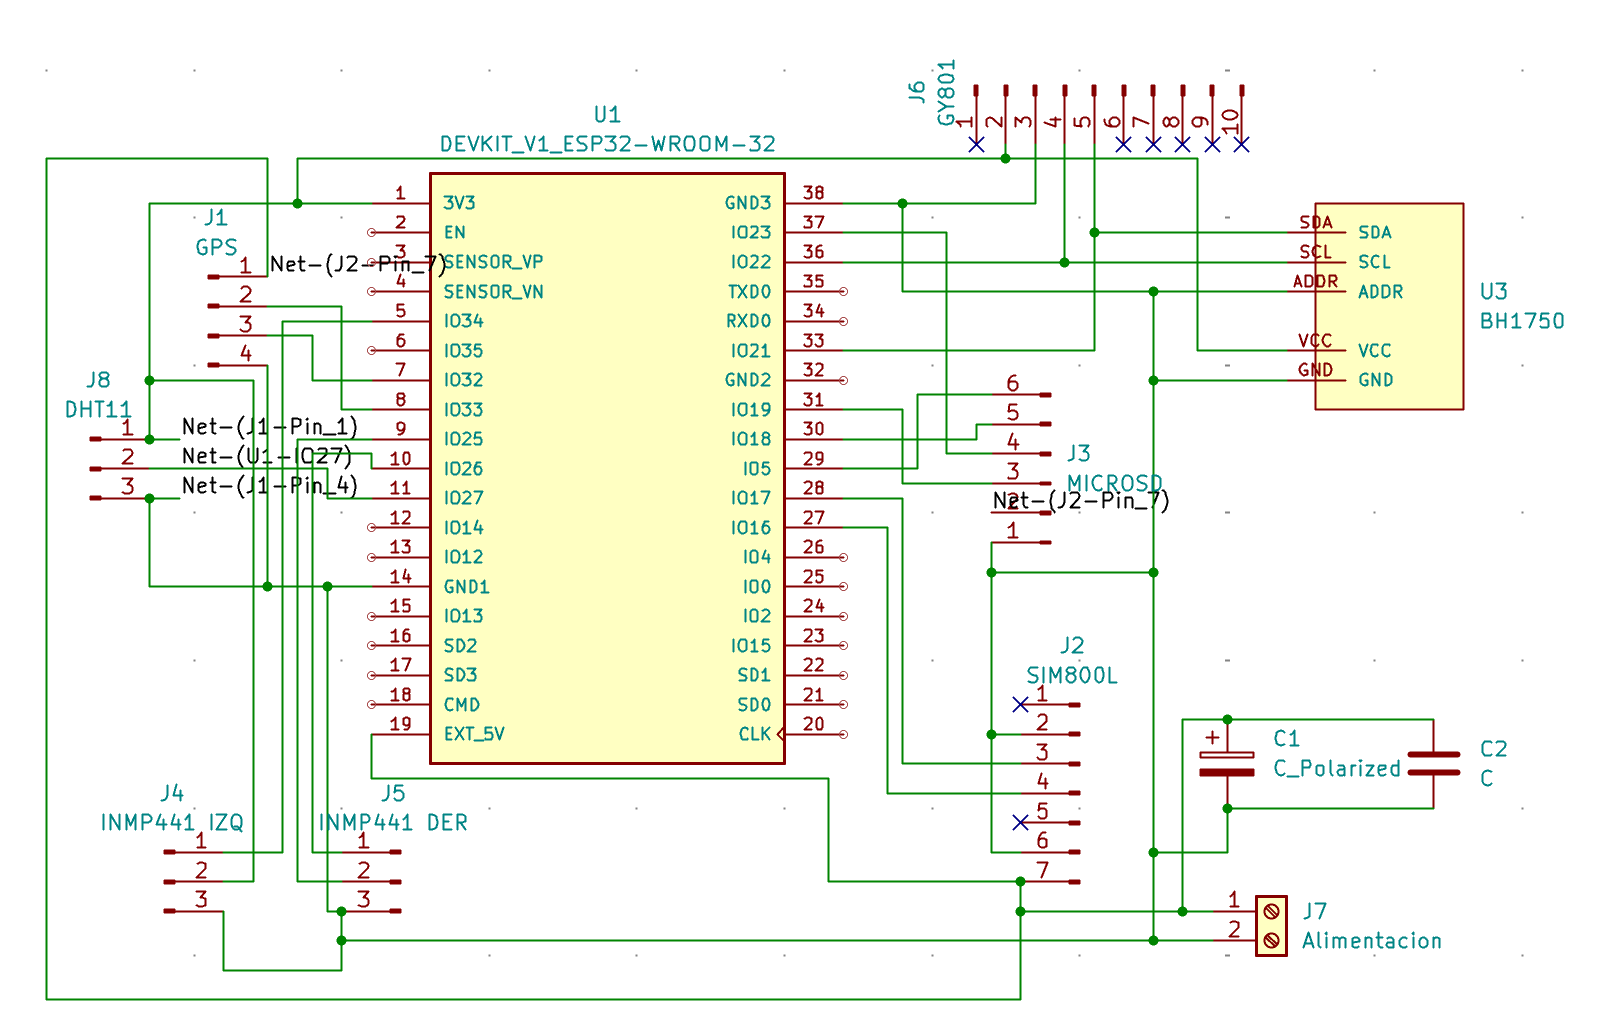
\includegraphics[width=0.98\textwidth,height=0.53\textheight,keepaspectratio]{01_esquematico_kicad.png}
  \caption{Esquemático general de la portadora realizado en KiCad. Se distinguen
  U1, los headers de sensores, J7 de alimentación y los condensadores de reserva.}
  \label{fig:esquematico}
\end{figure}

Las etiquetas del esquema se contrastaron con el firmware: GPS en GPIO32/33,
I2C en GPIO21/22, SPI en GPIO18/19/23/5, UART1 del módem en GPIO16/17, DHT11 en
GPIO27 e I2S del micrófono en GPIO26/25/34. Esta trazabilidad evita que una pista
correctamente dibujada termine conectada a una etiqueta \codigo{Dxx} diferente en
otra versión de DevKit.

\section{Placement y routing}

La distribución física se organizó por zonas. El ESP32 ocupa el centro y conserva
libre el extremo de su antena; los headers de sensores se acercan al perímetro; la
alimentación se agrupa junto a la bornera; y la zona de microSD/SIM se deja accesible
para retirar módulos y cables. En el diseño se mantuvieron las siguientes reglas:

\begin{itemize}
  \item plano de GND continuo en la cara de retorno siempre que no invada una zona
        de antena o un recorte mecánico;
  \item pistas de alimentación más anchas que las señales y trayectos cortos para
        la rama de corriente pulsante del SIM800L;
  \item I2C, SPI y UART alejados de la rama celular y del inductor de un regulador;
  \item \codigo{SD\_CS} con pull-up de 10 k$\Omega$ a 3,3 V para que el pin de
        arranque permanezca alto;
  \item puntos de acceso y serigrafía orientados para que el cableado pueda
        realizarse sin consultar continuamente el código.
\end{itemize}

\begin{figure}[H]
  \centering
  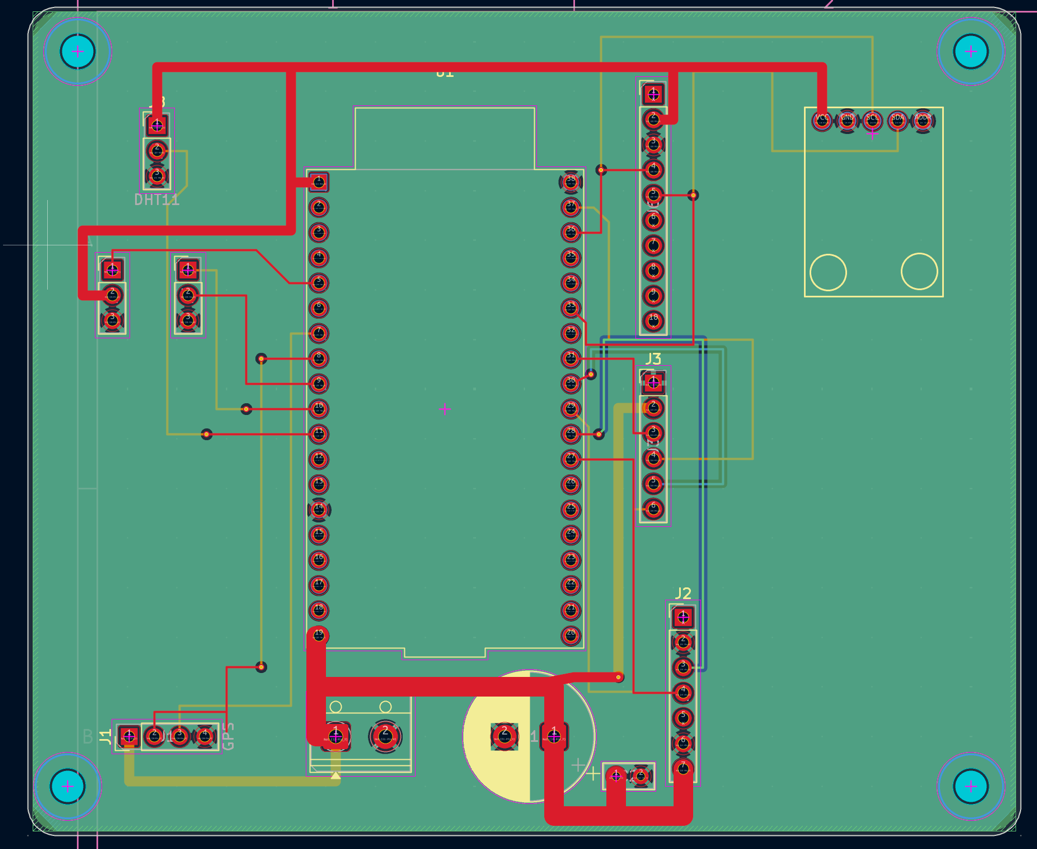
\includegraphics[width=0.91\textwidth,height=0.61\textheight,keepaspectratio]{02_layout_pcb_kicad.png}
  \caption{Vista de placement y routing de la PCB. La geometría deja el ESP32 en
  la zona central y distribuye los conectores alrededor de los bordes.}
  \label{fig:layout}
\end{figure}

La vista de layout fue útil para detectar cruces de conductores, orientar el pin 1
de los headers y revisar la posición de los cuatro agujeros de montaje. También
permitió comprobar que el USB, la tarjeta microSD y las antenas no quedaran
bloqueados por una pared de la caja.

\section{Footprints, serigrafía y revisión previa}

Los footprints de la portadora se eligieron para headers de paso de 2,54 mm y para
la variante de DevKit realmente disponible. Antes de generar los archivos de
fabricación se revisaron:

\begin{enumerate}
  \item correspondencia pin--net entre el esquemático y el layout;
  \item polaridad de C1, bornera J7 y conectores de alimentación;
  \item separación de los keepouts de antena, micrófono y magnetómetro;
  \item taladros de montaje, orientación del pin 1 y acceso del USB;
  \item reglas ERC/DRC y coherencia entre Gerbers, taladros y lista de materiales.
\end{enumerate}

La serigrafía conserva las referencias de conectores y las funciones de las
interfaces. Para una siguiente revisión se mantienen como mejoras recomendadas
la incorporación de más puntos de prueba, la confirmación de la huella exacta de
cada breakout y el marcado visible de advertencias de 3,3 V y de la rama SIM800L.

% -----------------------------------------------------------------------------
\chapter{Fabricación y ensamblaje de la PCB}
% -----------------------------------------------------------------------------

\section{Orden de fabricación}

Los archivos de fabricación se generaron desde la revisión de KiCad que se muestra
en las figuras. La tarjeta se trató como una PCB portadora de cuatro capas, con
planos internos para alimentación y retorno, y capas externas para componentes y
señales. También se incorporaron máscara de soldadura y serigrafía para identificar
el cableado. La captura de seguimiento
del proveedor registra el avance del lote entre el 4 y el 7 de agosto de 2026.

\begin{figure}[H]
  \centering
  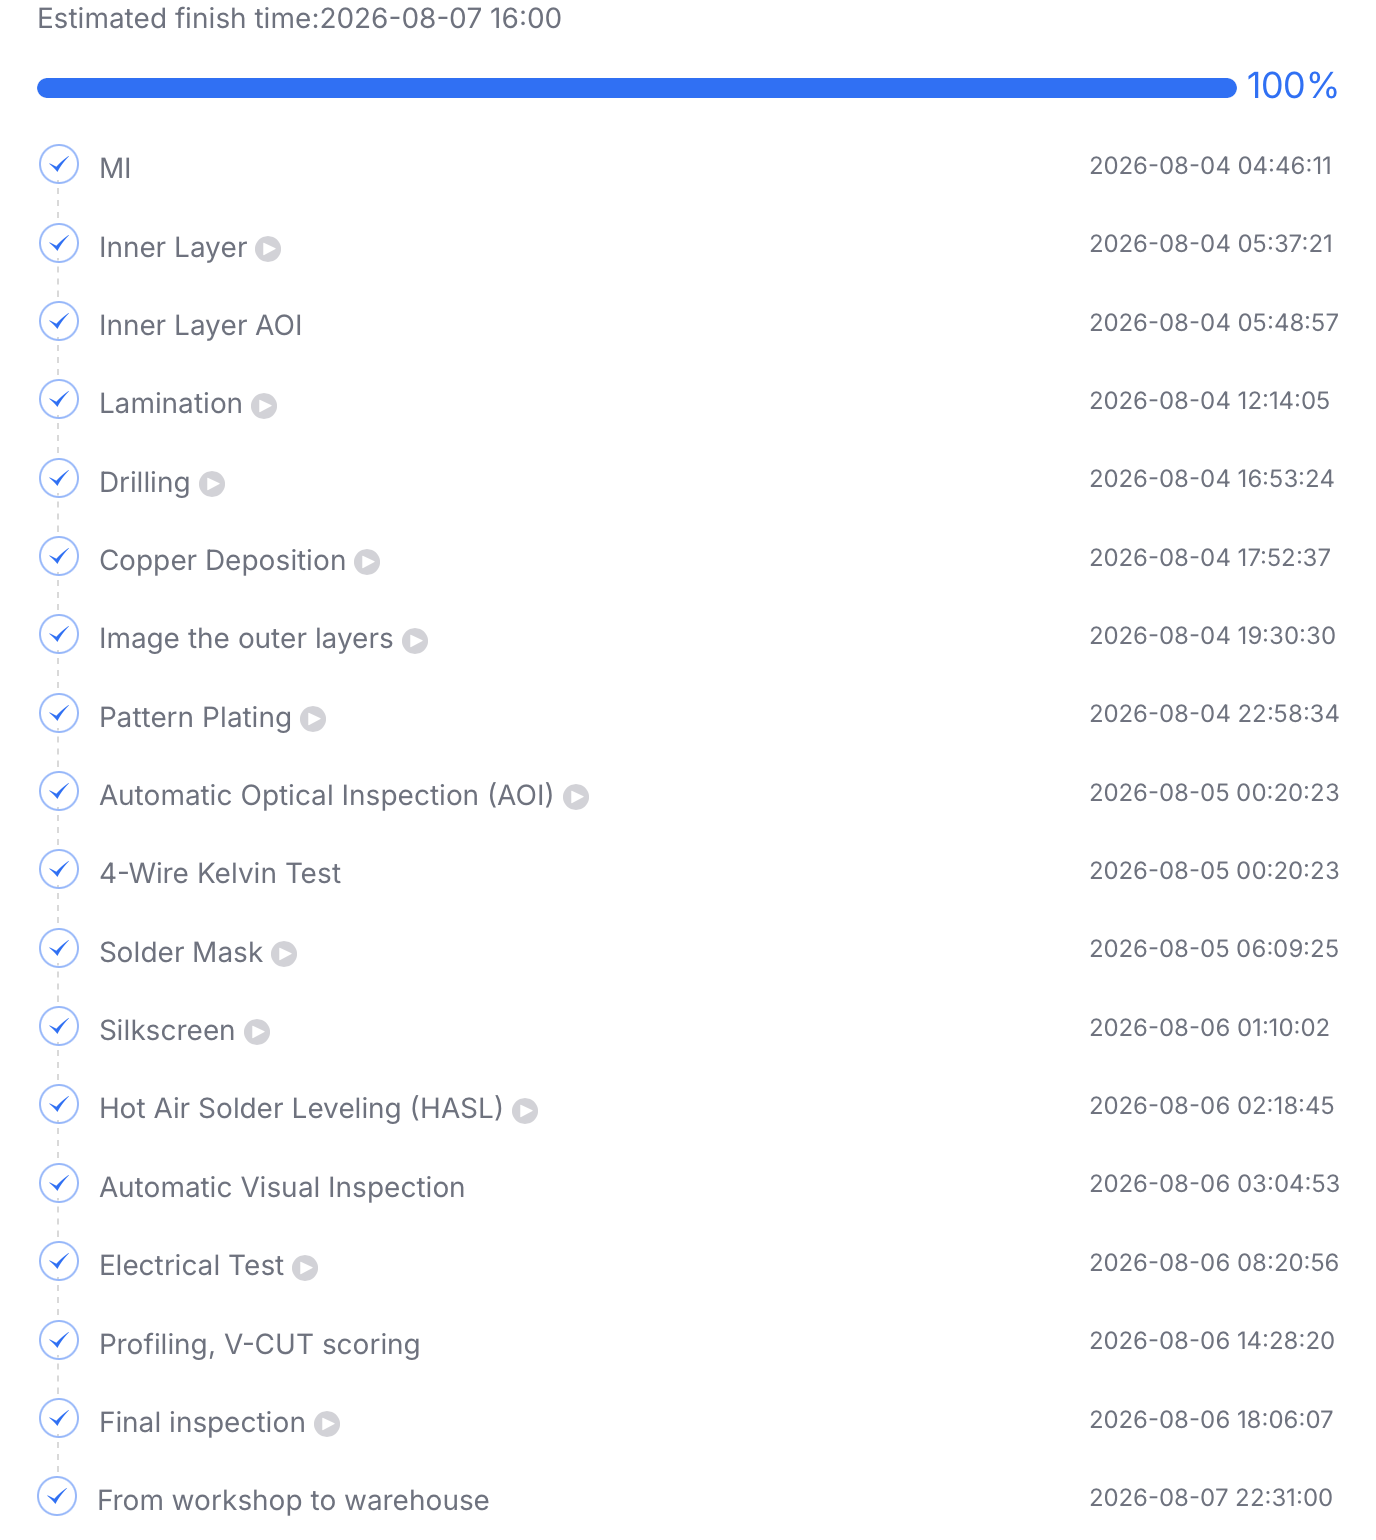
\includegraphics[height=0.67\textheight,width=0.78\textwidth,keepaspectratio]{03_fabricacion_jlcpcb.png}
  \caption{Seguimiento de fabricación del lote: laminación, taladrado, cobre,
  inspección óptica, prueba Kelvin, máscara, serigrafía, HASL, prueba eléctrica e
  inspección final.}
  \label{fig:jlcpcb}
\end{figure}

La secuencia observada es importante porque muestra que la fabricación no se
limitó a exportar una imagen del layout: hubo generación de capas, taladros,
metalización, inspecciones y perfilado. Al recibir la tarjeta se compararon el
contorno, los agujeros, la máscara y la serigrafía con la vista de KiCad antes de
instalar los módulos.

\begin{figure}[H]
  \centering
  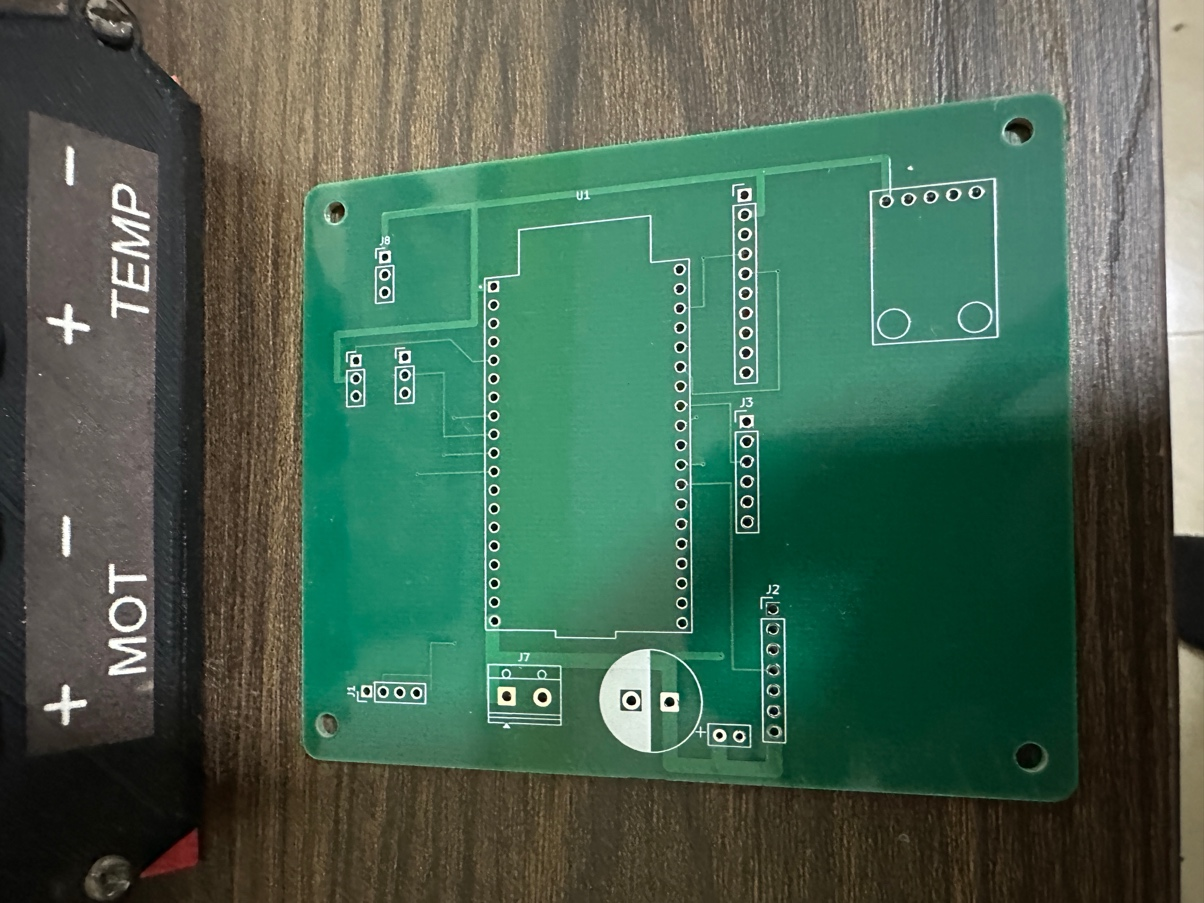
\includegraphics[width=0.78\textwidth,height=0.58\textheight,keepaspectratio]{04_pcb_desnuda.jpeg}
  \caption{PCB desnuda después de la fabricación. La máscara, los taladros de
  montaje, la serigrafía y las huellas de los headers se inspeccionaron antes de
  soldar.}
  \label{fig:pcbdesnuda}
\end{figure}

\section{Inspección de la placa desnuda}

La inspección de entrada se realizó sin alimentación. Se comprobó visualmente que
no hubiera delaminación, rebabas que impidieran insertar los headers, taladros
obstruidos o puentes evidentes entre pistas. Después se verificaron con multímetro
los puntos esenciales:

\begin{itemize}
  \item continuidad de GND entre los headers;
  \item ausencia de corto entre la entrada de energía y GND;
  \item aislamiento entre la rama de sensores y la rama del SIM800L;
  \item continuidad de las señales de cada bus hasta su GPIO;
  \item conexión de \codigo{MIC\_LR} a GND y de \codigo{BH\_ADDR} a la dirección
        seleccionada.
\end{itemize}

Esta etapa permite detectar un error de fabricación antes de que un módulo caro o
el ESP32 quede expuesto a una alimentación incorrecta.

\section{Soldadura y montaje de componentes}

La soldadura se ejecutó desde los elementos de menor altura hacia los de mayor
altura. Primero se instalaron headers, zócalos y la bornera; después se revisaron
las uniones y se montaron el capacitor electrolítico y los elementos de filtrado.
El ESP32 y los breakouts se dejaron desmontables para que las pruebas eléctricas y
el mantenimiento no exigieran desoldar la placa principal.

La inspección de las soldaduras consideró brillo, humectación, ausencia de puentes,
anclaje mecánico y orientación. En los headers se comprobó que la inserción fuera
perpendicular a la placa, ya que una inclinación pequeña puede impedir que un
módulo entre en la caja o cargar lateralmente sus pines.

\begin{figure}[H]
  \centering
  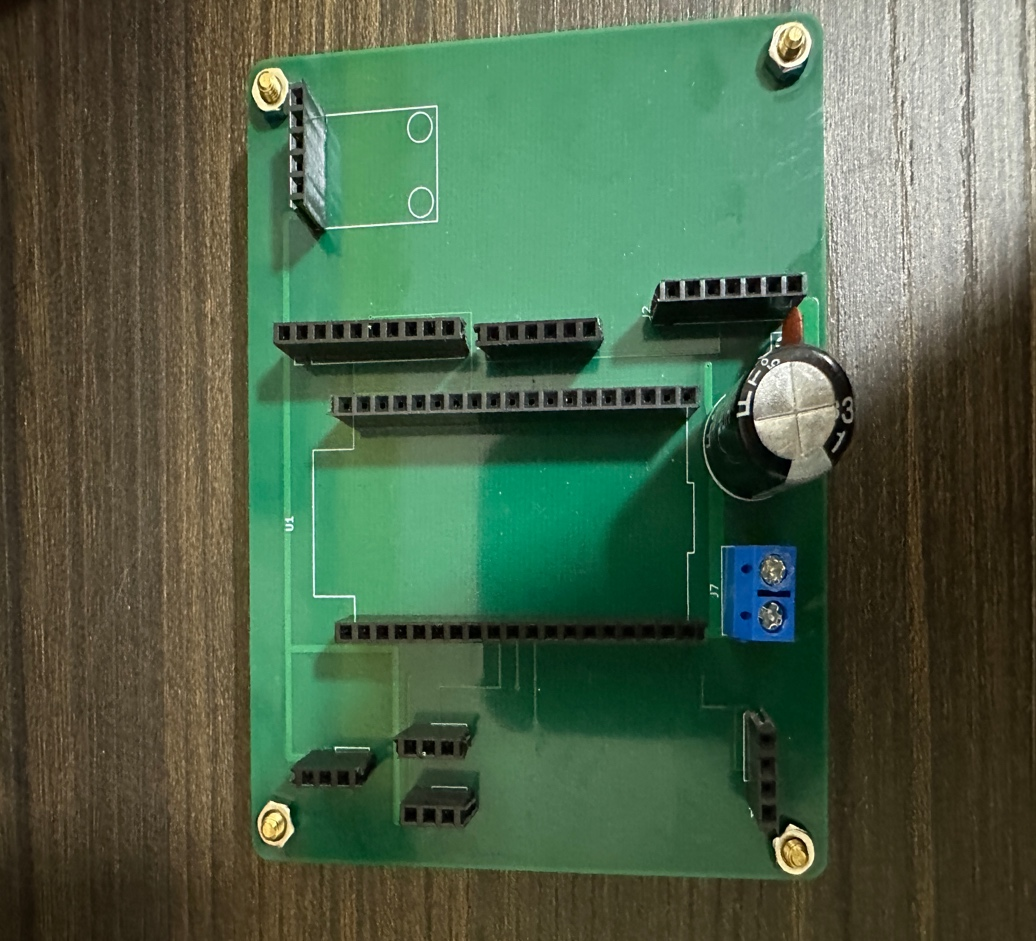
\includegraphics[width=0.78\textwidth,height=0.58\textheight,keepaspectratio]{04_pcb_ensamblada.jpeg}
  \caption{PCB con headers, bornera de alimentación y capacitor montados. La
  arquitectura modular permite insertar el ESP32 y los sensores después de la
  comprobación eléctrica inicial.}
  \label{fig:pcbensamblada}
\end{figure}

\begin{figure}[H]
  \centering
  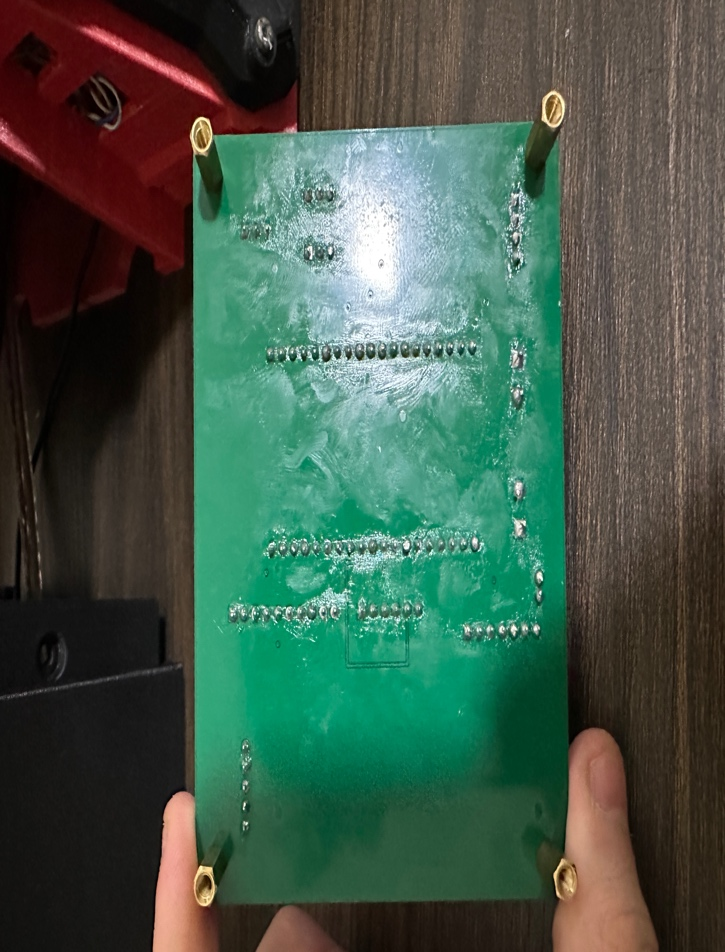
\includegraphics[width=0.72\textwidth,height=0.56\textheight,keepaspectratio]{06_pcb_soldadura_inferior.jpeg}
  \caption{Cara inferior de la PCB durante la inspección de soldaduras. Se
  revisaron continuidad, humectación y ausencia de puentes en las filas de pines.}
  \label{fig:soldadurainferior}
\end{figure}

\begin{figure}[H]
  \centering
  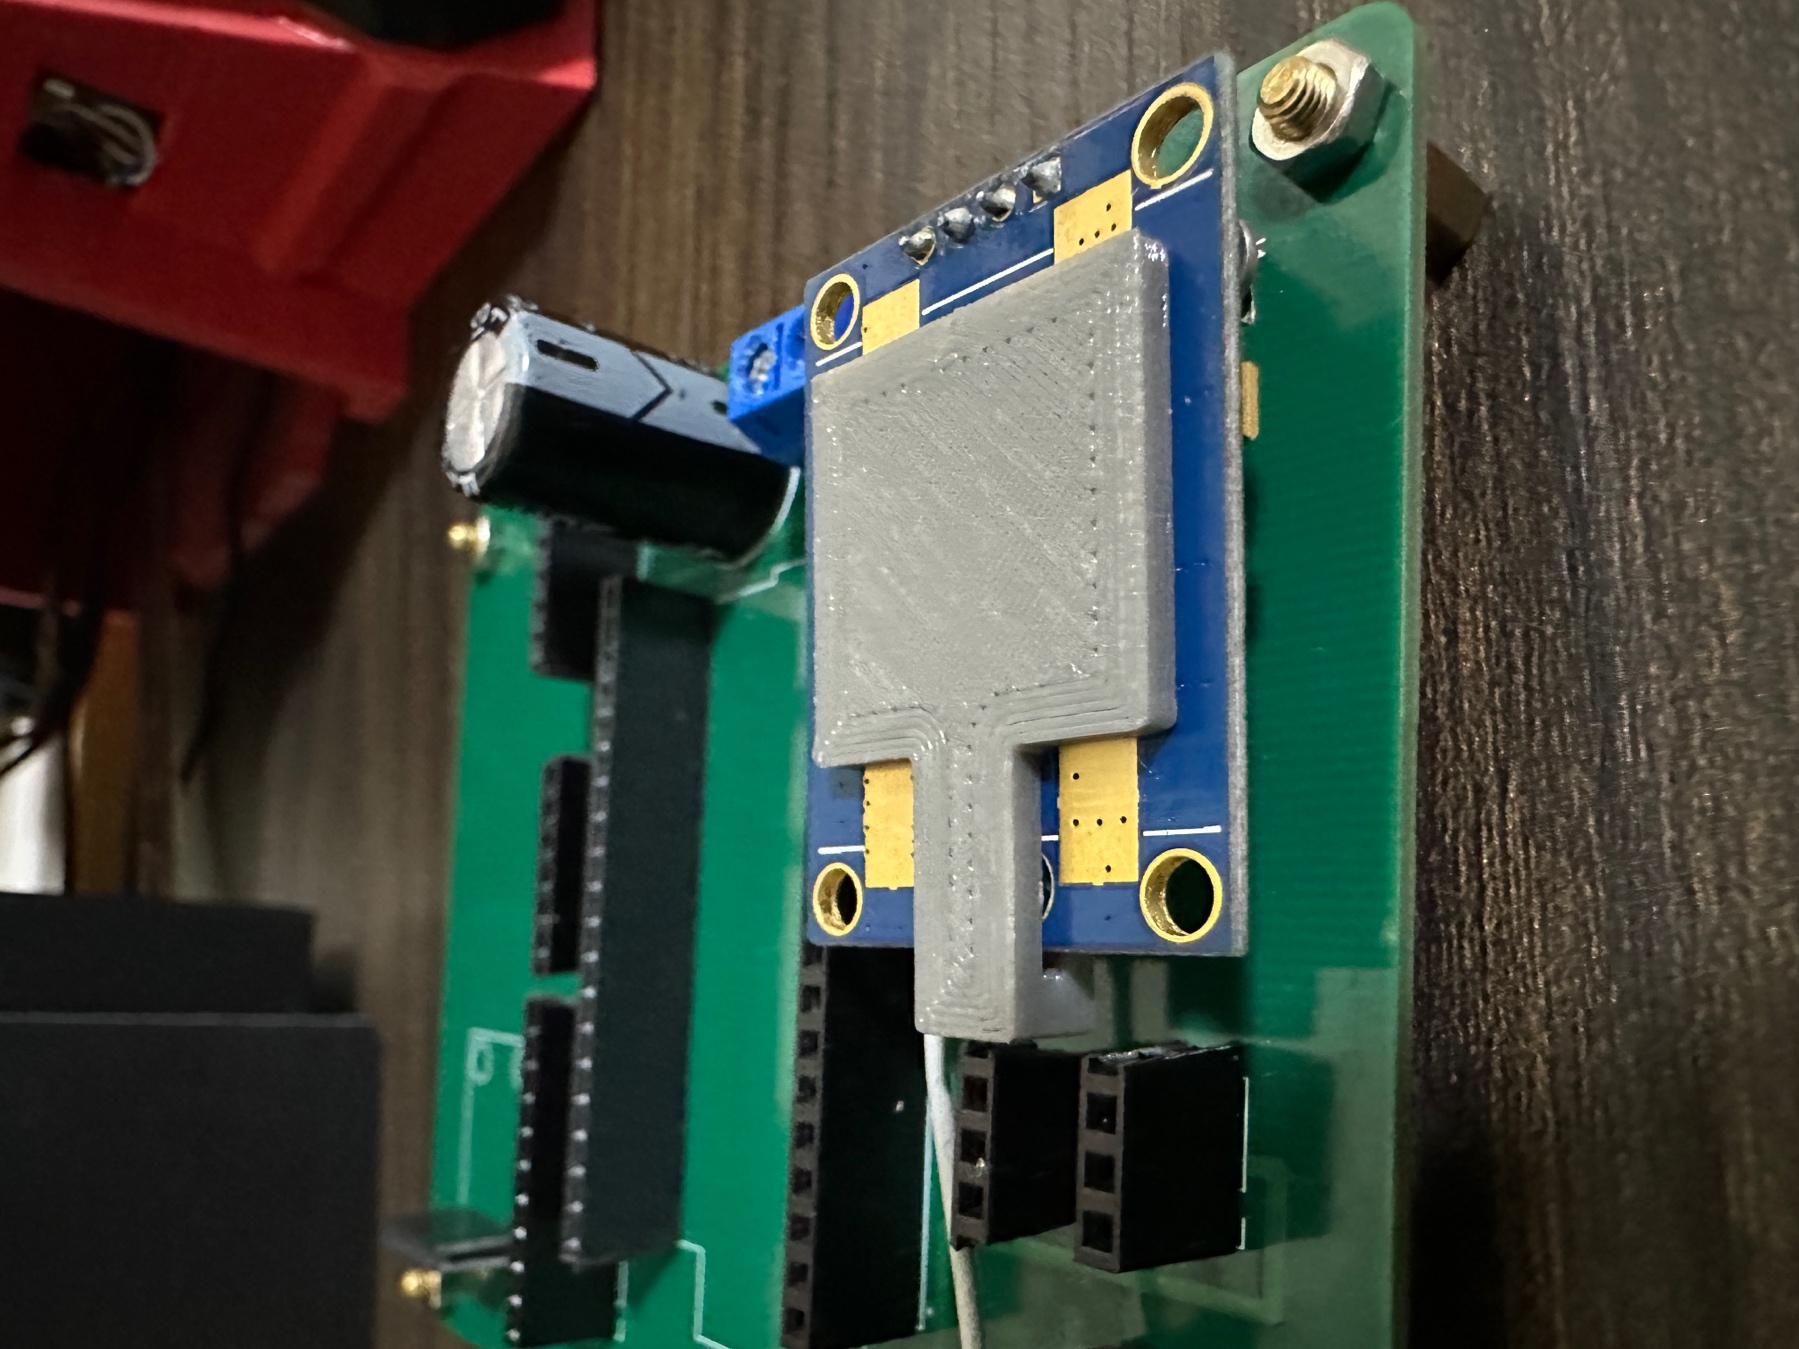
\includegraphics[width=0.76\textwidth,height=0.56\textheight,keepaspectratio]{07_detalle_gps.jpeg}
  \caption{Detalle del módulo GPS y del área de conectores. La posición deja
  accesibles los headers y separa el receptor de las zonas de potencia y RF.}
  \label{fig:detallegps}
\end{figure}

\section{Bring-up de la placa}

El bring-up se planificó de manera incremental para aislar fallos. El orden usado
para el montaje funcional es:

\begin{enumerate}
  \item alimentar la placa sin módulos y medir los rails;
  \item insertar el ESP32, abrir el monitor serial y confirmar que no hay reinicios;
  \item incorporar DHT11 y GPS, comprobando GPIO27 y UART2;
  \item incorporar el bus I2C y observar primero el scanner, luego cada dispositivo
        del GY-801 y el BH1750;
  \item probar microSD en SPI y verificar montaje, escritura JSONL y recuperación;
  \item probar el INMP441 con \codigo{L/R=GND}, manteniendo GPIO34 como entrada;
  \item evaluar el SIM800L solo con fuente independiente, antena y la secuencia AT,
        GPRS, MQTT y TLS definida en la documentación.
\end{enumerate}

Los environments de PlatformIO que materializan esta secuencia son
\codigo{test\_dht11}, \codigo{test\_gps}, \codigo{test\_i2c\_scanner},
\codigo{test\_gy801}, \codigo{test\_bh1750}, \codigo{test\_microsd},
\codigo{test\_inmp441} y, cuando corresponda, los de SIM800L. El perfil de
integración recomendado es \codigo{vehiclesense\_wifi}; la ruta celular permanece
experimental y no debe convertirse en un fallback inseguro.

% -----------------------------------------------------------------------------
\chapter{Diseño y fabricación de la caja}
% -----------------------------------------------------------------------------

\section{Criterios mecánicos}

La envolvente se diseñó alrededor del conjunto real, no de un rectángulo abstracto.
Los criterios que guiaron el modelado fueron:

\begin{itemize}
  \item base rígida con apoyos alineados con los agujeros de la PCB;
  \item paredes y tapa desmontables para mantenimiento;
  \item aberturas para USB, interruptor, alimentación y cables de sensores;
  \item ventilación lateral sin cubrir el interior con una pared continua;
  \item separación entre antenas, micrófono, módulo de luz y superficies que puedan
        alterar sus lecturas;
  \item holguras ajustadas mediante prueba de encaje de la pieza impresa, no por
        una cota histórica copiada de otra versión.
\end{itemize}

\section{Modelado CAD}

El modelo se construyó como una caja abierta con postes de fijación, recortes de
servicio y una tapa independiente. Las esquinas y los puntos de cierre se diseñaron
para guiar el armado, mientras que las rejillas laterales aportan ventilación y
permiten que el conjunto no quede completamente aislado del ambiente.

\begin{figure}[H]
  \centering
  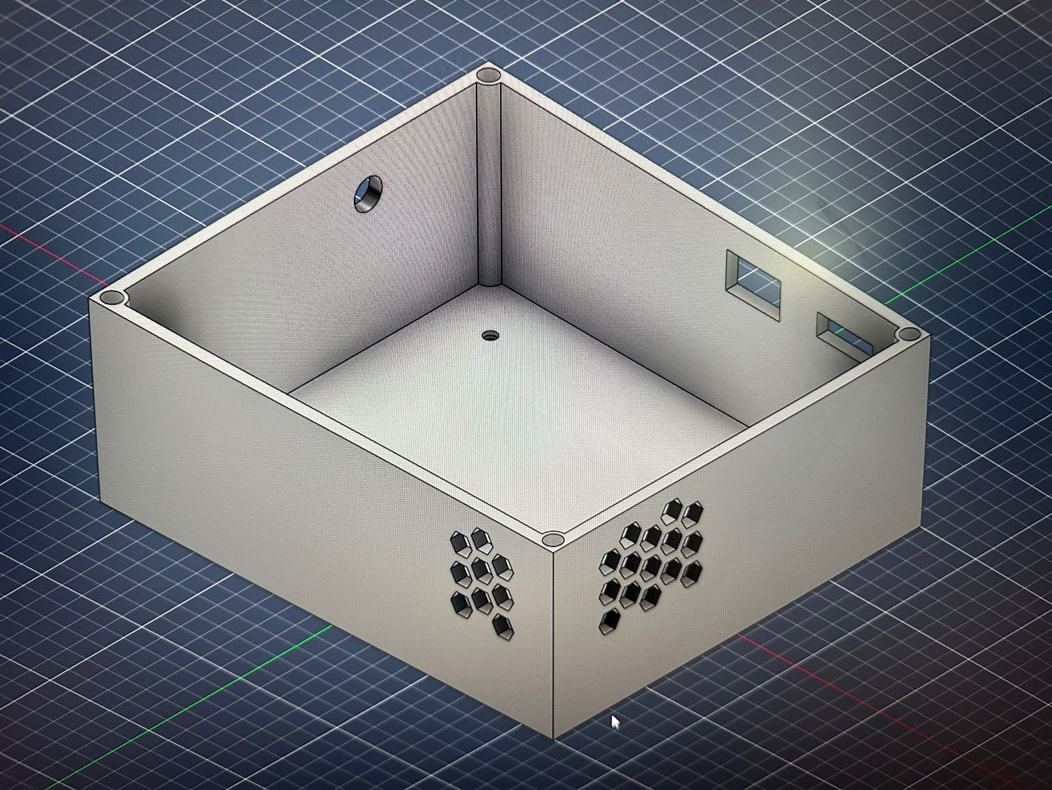
\includegraphics[width=0.94\textwidth,height=0.55\textheight,keepaspectratio]{05_caja_cad.jpeg}
  \caption{Modelo CAD de la caja PETG. Se observan los postes de fijación, la tapa
  desmontable, los recortes laterales y la ventilación tipo rejilla.}
  \label{fig:cajacad}
\end{figure}

En esta etapa también se verificó la orientación de la placa: el USB y la entrada
de alimentación deben coincidir con los recortes de la pared, el micrófono debe
conservar un puerto libre y la zona de la antena GPS no debe quedar debajo de una
superficie conductora.

\section{Impresión 3D en PETG}

Las piezas se fabricaron mediante FDM con filamento PETG. Se imprimieron la base y
la tapa como piezas separadas para simplificar la orientación sobre la cama, reducir
soportes y facilitar el mantenimiento. Una vez retirados los soportes y las rebabas,
se revisaron las caras de apoyo, los taladros y los bordes que entran en contacto
con la placa.

\begin{figure}[H]
  \centering
  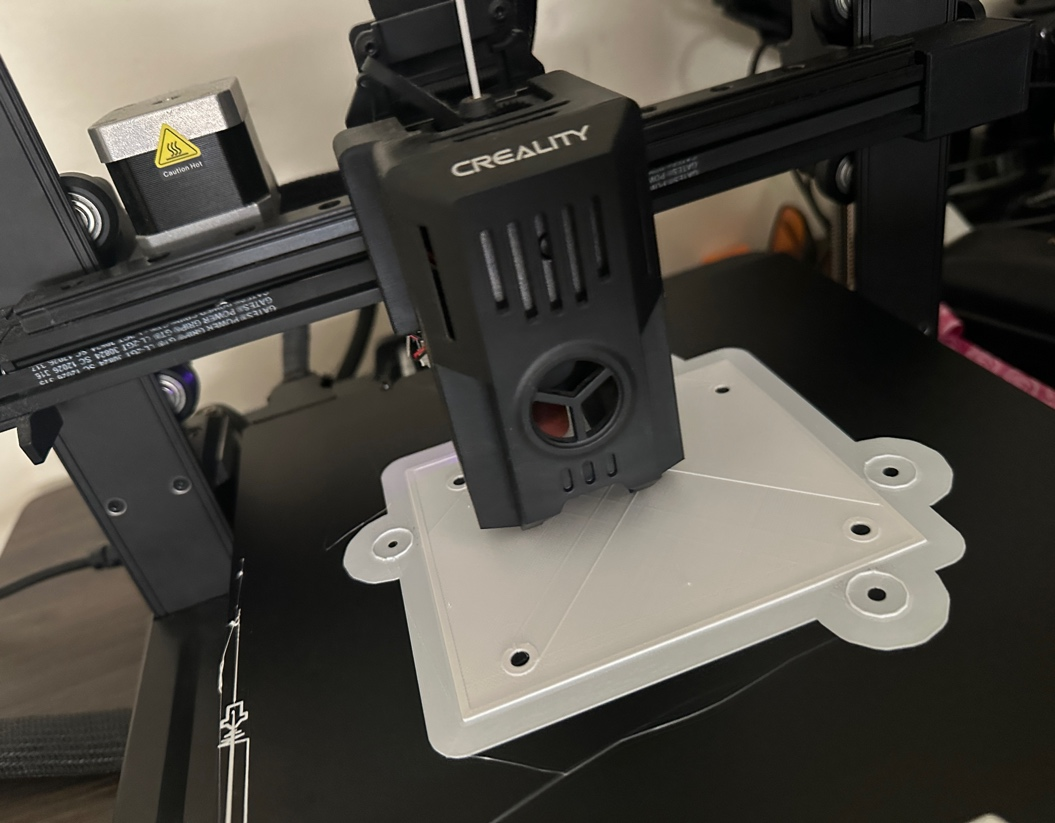
\includegraphics[width=0.78\textwidth,height=0.58\textheight,keepaspectratio]{09_impresion_caja.jpeg}
  \caption{Impresión FDM de una pieza de la caja en PETG. La orientación sobre la
  cama se eligió para conservar la geometría de los apoyos y facilitar el acabado.}
  \label{fig:impresioncaja}
\end{figure}

El acabado superficial visible en las fotografías conserva las líneas de capa del
proceso. Para el prototipo se priorizó la funcionalidad del encaje y la resistencia
de los postes sobre un acabado cosmético. En una iteración posterior puede mejorarse
la unión base--tapa y el sellado, pero cualquier material o tratamiento debe
mantener libres el micrófono, el sensor de luz y las antenas.

\begin{figure}[H]
  \centering
  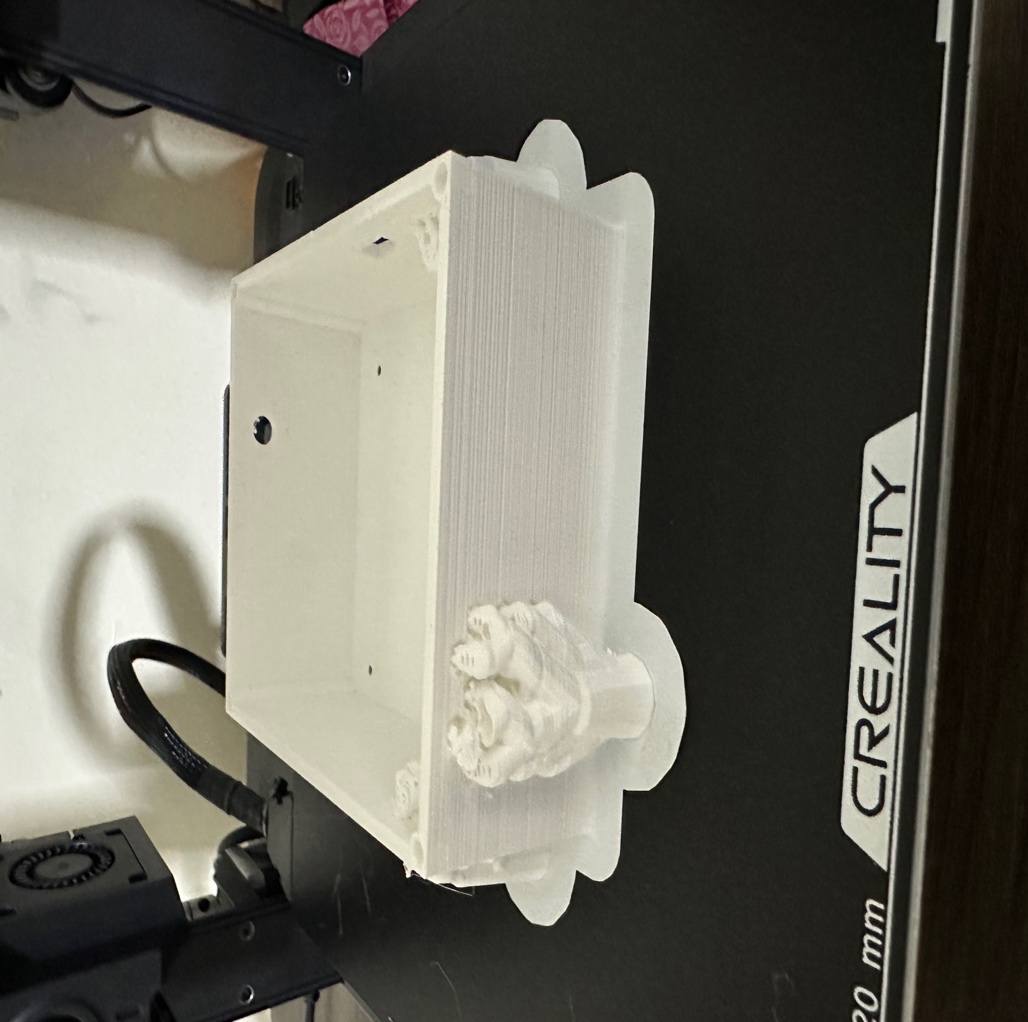
\includegraphics[width=0.77\textwidth,height=0.56\textheight,keepaspectratio]{10_caja_impresa.jpeg}
  \caption{Caja PETG impresa antes de introducir la electrónica. Se observan las
  paredes, los postes de fijación y los recortes que luego se alinean con la PCB.}
  \label{fig:cajaimpresa}
\end{figure}

\section{Comprobación de encaje}

La caja se probó primero sin cerrar completamente, con la PCB sostenida por
separadores. Se verificó que:

\begin{enumerate}
  \item la tarjeta se apoyara en los cuatro puntos sin flexión apreciable;
  \item ningún header quedara presionado contra una pared;
  \item los cables pudieran curvarse sin cargar sus soldaduras;
  \item el capacitor y los módulos altos quedaran libres de la tapa;
  \item los recortes frontales coincidieran con el USB y el interruptor;
  \item la ventilación no quedara tapada por el lugar de instalación.
\end{enumerate}

La ausencia de cotas en este informe no elimina este control: el criterio de
aceptación es que la pieza impresa vigente funcione con el hardware vigente. Si se
cambia de DevKit, breakout o módulo de antena, se debe repetir el ajuste del CAD y
la prueba de encaje.

% -----------------------------------------------------------------------------
\chapter{Montaje final e integración}
% -----------------------------------------------------------------------------

\section{Secuencia de montaje}

El montaje final se realizó en el siguiente orden:

\begin{enumerate}
  \item limpiar la caja y verificar que no quedaran partículas de impresión;
  \item instalar los separadores y comprobar que los agujeros de la PCB no tuvieran
        rebabas;
  \item fijar la placa sin forzarla y dejar el USB orientado hacia el recorte;
  \item insertar el ESP32, los headers y los módulos de sensores;
  \item ubicar GPS y micrófono en las zonas previstas, evitando doblar sus cables;
  \item conectar alimentación y señales siguiendo la serigrafía y \codigo{wiring.md};
  \item realizar el bring-up con la caja abierta;
  \item cerrar la tapa únicamente después de comprobar que no existe presión sobre
        cables, antenas, conectores o el capacitor.
\end{enumerate}

\section{Organización del cableado}

Los conductores se agruparon por función: potencia y GND por una ruta corta, I2C
separado de la rama pulsante del módem, SPI de la microSD cercano a su conector,
UART del GPS hacia el borde y señales I2S alejadas de los cables de corriente. Todos
los módulos comparten GND, pero el SIM800L conserva su fuente independiente. El
resultado reduce el esfuerzo sobre los headers y deja una ruta clara para retirar un
módulo durante el servicio.

\begin{evidenciabox}
\textbf{Regla de mantenimiento.} Antes de insertar, retirar o mover un módulo se
desconecta la alimentación. Después de una modificación se repite la prueba de
continuidad y se comprueba que ningún GPIO haya quedado expuesto a 5 V.
\end{evidenciabox}

\section{Acceso y servicio}

La caja no se trató como un encapsulado sellado. El USB y el interruptor se dejaron
al frente; las aberturas laterales permiten conducir sensores o una alimentación
externa; y la tapa desmontable permite revisar soldaduras, tarjeta microSD y
conectores. Esta decisión es apropiada para un prototipo académico porque facilita
la iteración, aunque no equivale a una clasificación IP ni a una validación de
vibración, humedad o temperatura de habitáculo.

\begin{figure}[H]
  \centering
  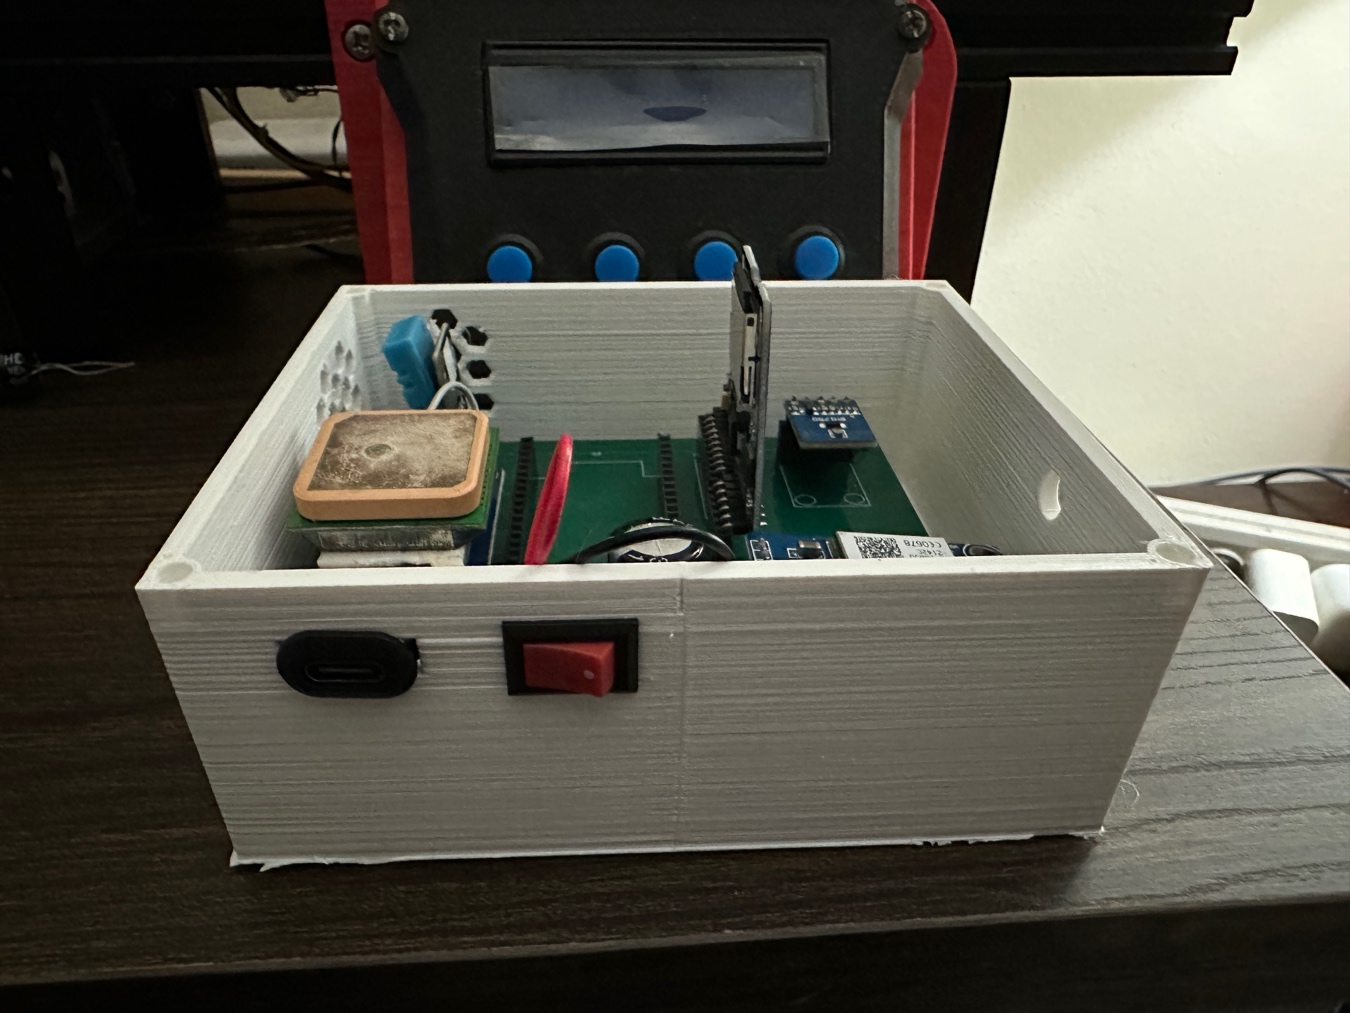
\includegraphics[width=0.94\textwidth,height=0.58\textheight,keepaspectratio]{06_montaje_final.jpeg}
  \caption{Montaje final con la PCB y los módulos dentro de la caja PETG. La vista
  abierta permite comprobar el encaje, el acceso frontal y la distribución del
  cableado.}
  \label{fig:montajefinal}
\end{figure}

La fotografía se tomó con la caja abierta para mostrar el interior. En operación
se puede colocar la tapa, pero el conjunto debe conservar el espacio libre de las
antenas y la ventilación diseñada. El cierre no debe utilizarse para compensar una
interferencia mecánica: si un módulo toca la tapa, se corrige el CAD o su posición.

% -----------------------------------------------------------------------------
\chapter{Validación y resultados}
\label{chap:validacion}
% -----------------------------------------------------------------------------

\section{Matriz de evidencias}

La tabla~\ref{tab:evidencias} separa lo que queda documentado por el diseño, lo
que se observa físicamente y lo que todavía requiere un registro de medición.

\begin{table}[H]
\centering
\small
\caption{Evidencia disponible para la revisión del conjunto.}
\label{tab:evidencias}
\begin{tabularx}{\textwidth}{>{\bfseries}p{3.5cm} p{2.8cm} X}
\toprule
Elemento & Estado & Evidencia y límite \\
\midrule
Esquemático y netlist & \implementado & Figura~\ref{fig:esquematico} y contraste con \codigo{pins.h}; se debe repetir ERC si cambia un módulo. \\
Layout de la PCB & \implementado & Figura~\ref{fig:layout}; placement, routing, serigrafía y agujeros visibles. \\
Fabricación del lote & \visual & Figura~\ref{fig:jlcpcb} registra las etapas del proveedor y la figura~\ref{fig:pcbdesnuda} muestra la tarjeta recibida; las imágenes no sustituyen un certificado de lote. \\
Soldadura y headers & \visual & Figuras~\ref{fig:pcbensamblada}--\ref{fig:soldadurainferior}; revisión visual de uniones, polaridad y fijación mecánica. \\
Módulos y conectores & \visual & Figura~\ref{fig:detallegps}; se revisó la posición del GPS y el acceso a los headers. \\
Caja PETG & \visual & Figuras~\ref{fig:cajacad}--\ref{fig:cajaimpresa} y figura~\ref{fig:montajefinal}; CAD, impresión y encaje de la pieza vigente. \\
Firmware y perfiles & \automatico & PlatformIO define diagnósticos independientes y pruebas nativas; compilar no demuestra el sensor conectado. \\
Precisión y estabilidad en vehículo & \pendiente & Requiere ensayo prolongado con sensores, vibración, temperatura, alimentación y fallos inducidos. \\
\bottomrule
\end{tabularx}
\end{table}

\section{Lista de aceptación del ensamblaje}

El conjunto se considera correctamente ensamblado cuando se cumplen estos puntos:

\begin{itemize}
  \item la PCB queda apoyada en sus puntos de fijación sin flexión ni contacto con
        la pared;
  \item el ESP32 puede retirarse de sus zócalos y el USB permanece accesible;
  \item la serigrafía permite identificar J-DHT, J-GPS, J-GY801, J-BH1750, J-SD,
        J-SIM, J-MIC y J-PWR;
  \item no hay puentes de soldadura visibles ni pines doblados;
  \item la continuidad de GND y el aislamiento de las ramas de alimentación son
        correctos antes de energizar;
  \item la rama del SIM800L no toma corriente del rail de 3,3 V del ESP32;
  \item las aberturas de USB, alimentación, antena, micrófono y ventilación no están
        bloqueadas;
  \item la tapa puede desmontarse sin arrancar cables ni ejercer presión sobre los
        módulos.
\end{itemize}

% -----------------------------------------------------------------------------
\chapter{Conclusiones}
% -----------------------------------------------------------------------------

Se completó una cadena coherente de diseño y fabricación para el nodo embarcado.
El esquemático de KiCad traduce las interfaces del firmware a conectores físicos;
el layout coloca el ESP32, sensores, almacenamiento, alimentación y comunicación
en una portadora modular; el lote fabricado incorpora máscara, serigrafía y
taladros de montaje; y la soldadura deja los módulos reemplazables para el bring-up.

La caja PETG aporta una segunda capa de integración: fija la PCB con separadores,
protege los headers, ofrece acceso frontal a USB y alimentación, y conserva
ventilación y zonas libres para antenas y sensores. El ajuste se verificó sobre la
pieza vigente y no se mezclaron cotas antiguas en el texto.

El resultado es un prototipo físico ordenado y mantenible, listo para completar la
validación funcional por sensor y la prueba prolongada en el vehículo. Antes de
considerar una revisión para uso real deben repetirse el análisis de alimentación,
la protección de entrada, las pruebas de vibración/temperatura y la calibración de
los sensores en su posición definitiva.

\end{document}
